%%%%%%%%%%%%%%%%%%%%%%%%%%%%%%%%%%%%%%%%%%%%%%%%%%%%%%%%%%%
% start the content of the presentation
\subsection{Broad Goals of Uncertainty Quantification}
%%%%%%%%%%%%%%%%%%%%%%%%%%%%%%%%%%%%%%%%%%%%%%%%%%%%%%%%%%
\begin{frame}[t]

\begin{itemize}
	\item Quantify and reduce uncertainty
	\vskip 20pt
	\item Be \emph{accurate} and \emph{precise}
	\vskip 20pt
	\item Make inferences and predictions
	\vskip 20pt
	\item Design ``efficient'' experiments
	\vskip 20pt
	\item Collect and use data ``intelligently''
\end{itemize}

\end{frame}

\subsection{Formal Definitions}
%%%%%%%%%%%%%%%%%%%%%%%%%%%%%%%%%%%%%%%%%%%%%%%%%%%%%%%%%%
\begin{frame}[t]
%\vskip 25pt
\centering
\begin{figure}
\centering

\begin{tikzpicture}[node distance=2cm, auto,]
 %nodes
 
 % We make a dummy figure to make everything look nice.
 \node[] (dummy) {};
  \node[right=of dummy] (data) {$\dspace$};
  
  \node[punkt, inner sep=5pt,below=of dummy]
 (model) {Model \\ (PDE)}
 	edge[pil,->, bend right=25] node[right] {$Q(u\lam)$} (data);

 \node[left=of dummy] (pspace) {$\Lambda$}
   edge[pil,->, bend right=45] node[left] {$u\lam$} (model)
   edge[pil,->, bend left=45] node[above] {$Q\lam$} (data);
   
   
\end{tikzpicture}

\vspace{1em}
\emph{Defining the Quantity of Interest Map}
\end{figure}

\end{frame}


%%%%%%%%%%%%%%%%%%%%%%%%%%%%%%%%%%%%%%%%%%%%%%%%%%%%%%%%%%
\begin{frame}{The QoI Map}

\only<1>{

\begin{figure}[h]
	\includegraphics[width=0.85\textwidth]{./figures/threelevels/schematic_lambda_solution_data}
\end{figure}

}

\only<2>{

\begin{figure}[h]
	\includegraphics[width=0.85\textwidth]{./figures/threelevels/schematic_lambda_data}
\end{figure}

}

\only<3>{

\begin{figure}[h]
	\includegraphics[width=0.85\textwidth]{./figures/threelevels/schematic_lambda_data_level1}
\end{figure}

}

\end{frame}

%%%%%%%%%%%%%%%%%%%%%%%%%%%%%%%%%%%%%%%%%%%%%%%%%%%%%%%%%%
\begin{frame}{A Forward UQ Problem}

\begin{figure}[h]
	\includegraphics[width=0.85\textwidth]{./figures/threelevels/schematic_lambda_data_level3}
\end{figure}

{We denote the measurable spaces of parameters and data on the QoI as $(\pspace,\pborel)$ and $(\dspace,\dborel)$, respectively.}
\bigskip

\tdeepred{Given some prior density $\pri$ on $(\pspace,\pborel)$, we let $\pfpr$ denote the push-forward of this density on $(\dspace,\dborel)$.}

\end{frame}

%%%%%%%%%%%%%%%%%%%%%%%%%%%%%%%%%%%%%%%%%%%%%%%%%%%%%%%%%%
\begin{frame}{The Inverse QoI Map}

\begin{figure}[h]
	\includegraphics[width=0.85\textwidth]{./figures/threelevels/schematic_data_lambda_level1}
\end{figure}

\end{frame}

%%%%%%%%%%%%%%%%%%%%%%%%%%%%%%%%%%%%%%%%%%%%%%%%%%%%%%%%%%
\begin{frame}{An Inverse UQ Problem}

\begin{figure}[h]
	\includegraphics[width=0.85\textwidth]{./figures/threelevels/schematic_data_lambda_level3}
\end{figure}

\tdeepred{Given $\obs$ on $(\dspace,\dborel)$, we let $\pos$ denote the pullback (consistent) density on $(\pspace,\pborel)$.}

\end{frame}


\subsection{Basic Assumptions \& Terminology}
%%%%%%%%%%%%%%%%%%%%%%%%%%%%%%%%%%%%%%%%%%%%%%%%%%%%%%%%%%
\begin{frame}[t]

\begin{itemize}[<+->]
	\item State variable: $u$ {\color{gray}(e.g. heat, energy, pressure, deflection)}
	\vskip 10pt
	\item<.-> Parameters: $\lambda$ {\color{gray}(e.g. source term, diffusion, boundary data)}
	\vskip 10pt
		\item Deterministic model: $\MMM (u, \lambda) = 0$, $$\MMM:\lambda \to u(\lambda)$$

	\item Quantity of Interest map \tdeepred{(QoI)} - at least pcw differentiable \vskip 5pt
		\begin{itemize}[<+->]
		\item Functional of the solution $$q: u(\lambda) \to \RR$$
		\item Can be vector valued $$Q = \mat{c}{q_1\\ q_2\\ \vdots \\ q_d}$$
		\item<.-> $Q(\lambda) := Q(u(\lambda))$
	\end{itemize}
	
\end{itemize}

\end{frame}


\subsection{The Stochastic Inverse Problem}
%%%%%%%%%%%%%%%%%%%%%%%%%%%%%%%%%%%%%%%%%%%%%%%%%%%%%%%%%%
\begin{frame}[t]

\begin{figure}
\centering
	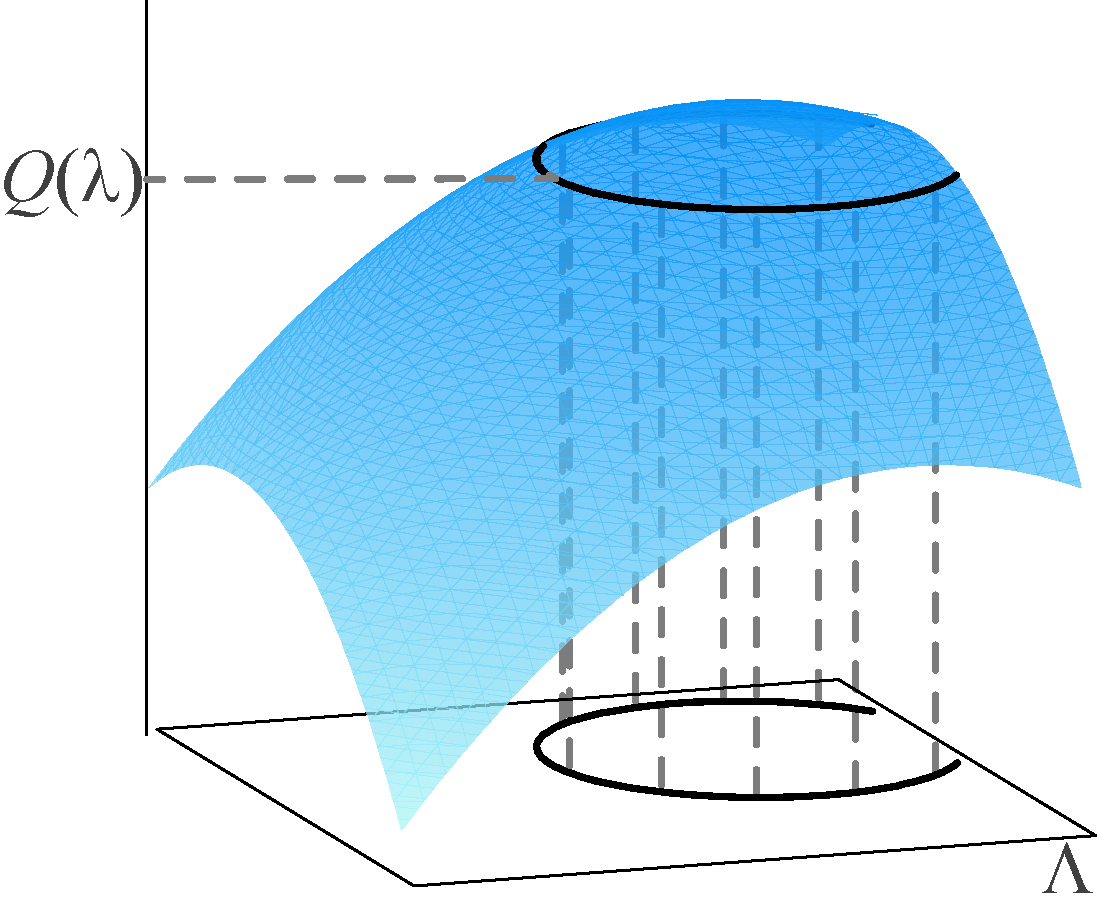
\includegraphics[width=.65\textwidth]{images/illustration1}<1>
	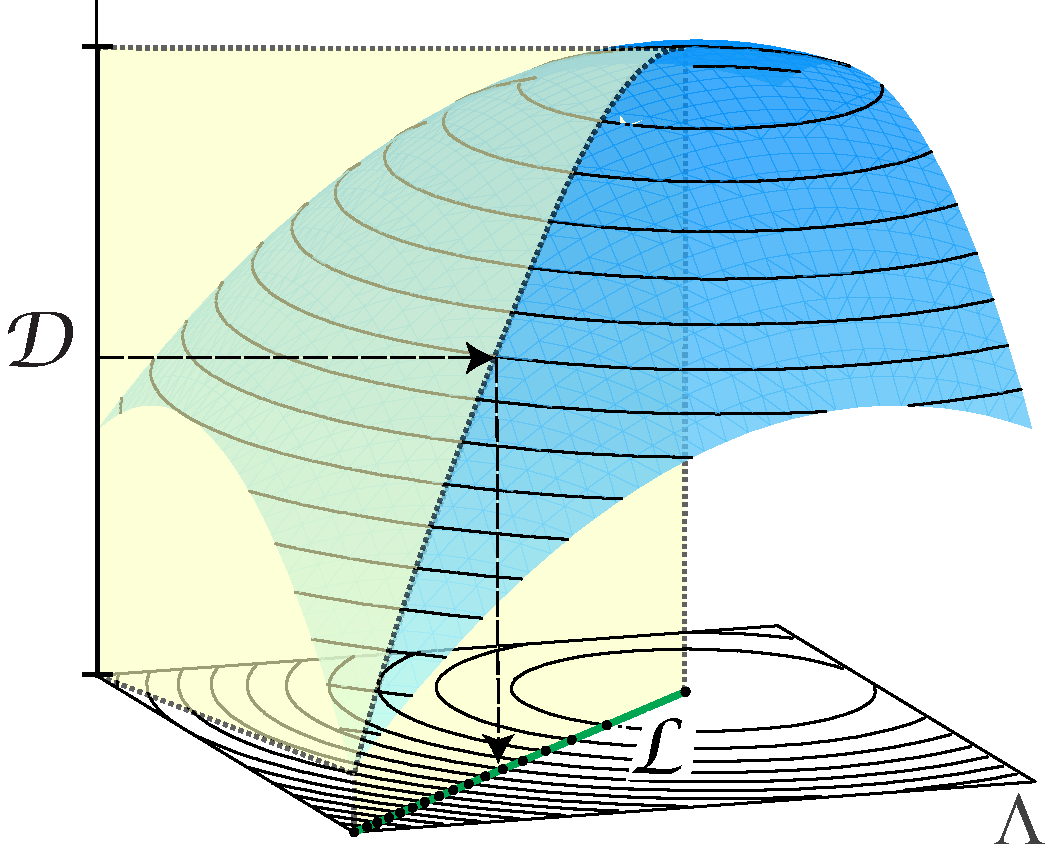
\includegraphics[width=.65\textwidth]{images/illustration2}<2>
	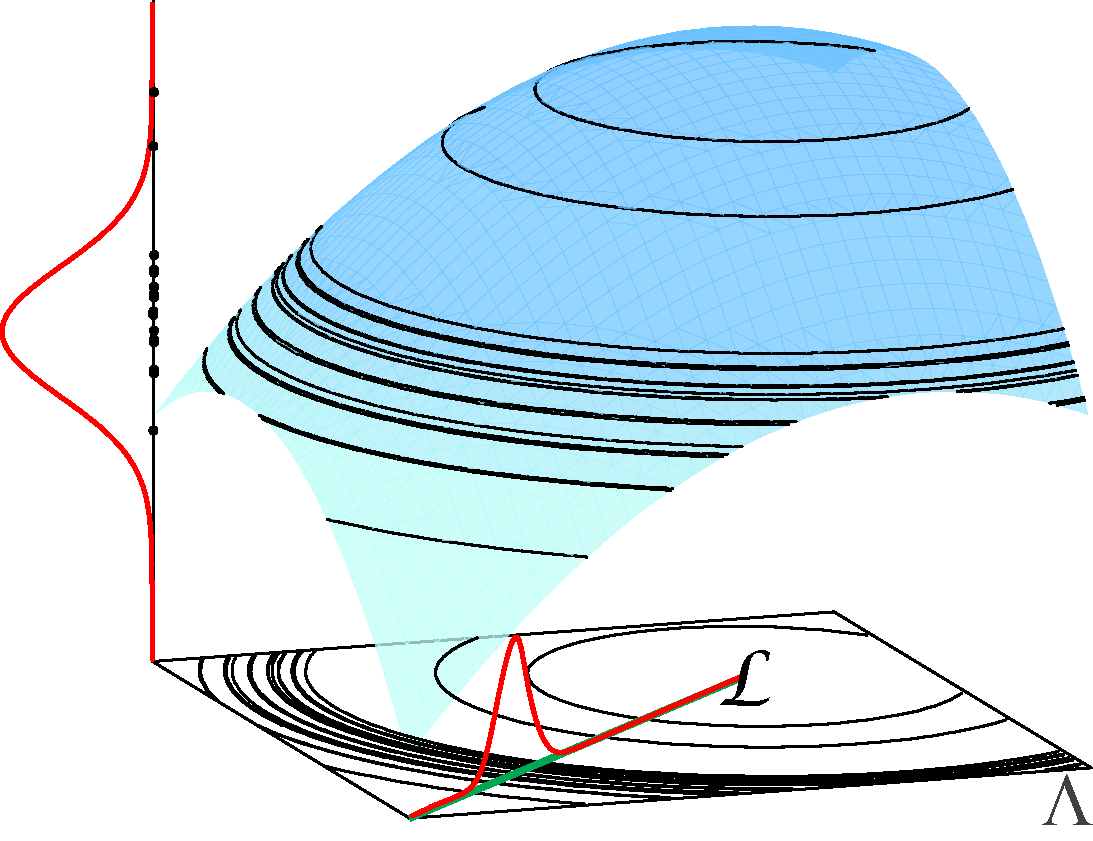
\includegraphics[width=.7\textwidth]{images/illustration3}<3>
\end{figure}
\begin{center}
{\scriptsize Figure adopted from \cite{BET14+} and used with permission}
\end{center}
\end{frame}

%%%%%%%%%%%%%%%%%%%%%%%%%%%%%%%%%%%%%%%%%%%%%%%%%%%%%%%%%%
\begin{frame}[t]

\begin{figure}
\centering
	\includegraphics[width=1\textwidth]{images/troy_mt3contour}
\end{figure}
\begin{center}

{\scriptsize Figure adopted from \cite{BET14+} and used with permission}

\tdeepred{Key Question:} Distinguish (assign probability to) events that belong to same contour. 
\end{center}
\end{frame}

\subsection{Problem Formulation and Solution}
%%%%%%%%%%%%%%%%%%%%%%%%%%%%%%%%%%%%%%%%%%%%%%%%%%%%%%%%%%%
\begin{frame}[t]

\begin{defn}[Inverse Problem]\label{defn:consistency}
Given $\observedP$ on $(\dspace, \dborel)$ the \textbf{inverse problem} is to determine a probability measure $\updatedP$ on $(\pspace, \pborel)$ such that 

	\begin{equation}\label{eq:inv}
		\updatedP(Q^{-1}(E)) = \observedP(E),
	\end{equation}
for all events $E \in \mathcal{B}_\dspace$, where

	\begin{equation*}
		\updated = \frac{d\updatedP}{d\mu_\pspace} \;\text{ and }\; \observed = \frac{d\observedP}{d\mu_\dspace}.
	\end{equation*}
\eqref{eq:inv} defines a \tdeepred{``Consistent Solution,''} yields a \tdeepred{Consistency Condition.}
\end{defn}

Note: {\scriptsize We use the notation $\PP$ and $\pi$ throughout this work to relate measures to their associated densities (i.e., Radon-Nikodym derivatives), which exist under the assumption of a dominating (Lebesgue) volume measure $\mu$.}
\end{frame}


%%%%%%%%%%%%%%%%%%%%%%%%%%%%%%%%%%%%%%%%%%%%%%%%%%%%%%%%%%
\begin{frame}[t]{Perspectives}
\begin{itemize}
	\item We seek the $\updatedP$ whose push-forward measure matches $\observedP$
	\item In measure-theoretic terms, $\updatedP$ is a pull-back measure of $\observedP$

	\begin{defn}[Observed Density]\label{defn:obsden}
		The density $\observed$ in \eqref{eq:inv} represents the uncertainty in QoI data.
	\end{defn}

	\begin{defn}[Initial Density]\label{defn:initialden}
		$\initial$ encodes prior beliefs about $\param$'s (before evidence is accounted for)
	\end{defn}

\end{itemize}

\end{frame}

%%%%%%%%%%%%%%%%%%%%%%%%%%%%%%%%%%%%%%%%%%%%%%%%%%%%%%%%%%
\begin{frame}[t]{Summarizing}
\begin{itemize}
	\item ``Push-forward'' \textbf{initial} beliefs using $\qoi$ to \textbf{compare} to \textbf{observed} (data)
	\item Solve forward problem to construct solution to inverse problem
	\item The push-forward density of $\initial$ under the map $\qoi$ is denoted by $\predicted$

	\begin{defn}[Predicted Density]\label{defn:predicted}
		$\predicted$ is given as the Radon-Nikodym derivative (with respect to $\mu_\dspace$) of the push-forward probability measure defined by:
		\begin{equation}\label{eq:pred}
			\predictedP (E)  = \initialP \left ( \qoi^{-1}(E) \right ), \; \forall \; E \in \dborel.
		\end{equation}
	\end{defn}

\end{itemize}

\end{frame}

%%%%%%%%%%%%%%%%%%%%%%%%%%%%%%%%%%%%%%%%%%%%%%%%%%%%%%%%%%
\begin{frame}[t]
These definitions are combined to form the \textbf{posterior density}, originally derived in \cite{BJW18}:
\begin{equation}\label{eq:post}
\predicted \lam = \initial \lam \frac{\pi_\dspace \q }{\predicted \q }, \; \lambda \in \pspace.
\end{equation}

\begin{itemize}
	\item $\obs$ and $\predicted$ defined on $(\dspace, \dborel)$ are evaluated at $\qlam$
	\item The map $Q$ impacts the structure of the posterior
	\item $\dspace$ itself depends on $Q$
	\item Primary work in solving for $\predicted$ (in \eqref{eq:inv}) requires constructing $\predicted$
	\item This is because $\initial$ and $\obs$ are given \emph{a priori} (often parametric)
	\item Posterior derived through use of Disintegration Theorem in \cite{BJW18}
	\item Existence and Uniqueness provided that we satisfy assumptions
\end{itemize}
\end{frame}



\subsection{Properties and Assumptions of the Posterior}
%%%%%%%%%%%%%%%%%%%%%%%%%%%%%%%%%%%%%%%%%%%%%%%%%%%%%%%%%%
\begin{frame}[t]
\begin{assumption}[Predictability Assumption]\label{as:pred}
The measure associated with $\obs$ is absolutely continuous with respect to the measure associated with $\obs$.
\end{assumption}


The requirement is guaranteed if the following is satisfied:
\begin{equation}\label{eq:pred}
\exists \; C>0 \text{ such that } \obs (d) \leq C \predicted(d) \text{ for a.e. } d\in \dspace,
\end{equation}
where it is understood that $d = Q\lam$ for some $\lambda \in \pspace$.
Assuming \eqref{eq:pred} holds, we restate the following theorem from \cite{BJW18}:
\begin{theorem}[Existence and Uniqueness]
For any set $A\in \pborel$, the solution $\predictedP$ given defined by
\begin{equation}\label{eq:cb_sol}
\predictedP (A) = \int_\dspace \left (  \int_{\pspace \in Q^{-1}(d)}  \initial\lam \frac{\obs\q}{\predicted\q} \, d\mu_{\pspace, d} \lam \right ) \, d\mu_\dspace(d), \; \forall \; A \in \pborel
\end{equation}
is a consistent solution, and is unique up to choice of $P_\pspace$ on $(\pspace, \pborel)$.
\end{theorem}

\end{frame}

%%%%%%%%%%%%%%%%%%%%%%%%%%%%%%%%%%%%%%%%%%%%%%%%%%%%%%%%%%
\begin{frame}[t]

This posterior density \eqref{eq:post} appearing within the iterated integral in \eqref{eq:cb_sol} has no normalization constant (it already integrates to one), which is summarized in Corollary 3.1 in \cite{BJW18} and restated in simplified form below:
\begin{corollary}\label{cor:int}
$\predictedP(\pspace) = 1$.
\end{corollary}

\end{frame}




%%%%%%%%%%%%%%%%%%%%%%%%%%%%%%%%%%%%%%%%%%%%%%%%%%%%%%%%%%
\begin{frame}[t]{Stability}

\begin{defn}{Total Variation / Statistical Distance}
	\begin{equation}\label{eq:tv}
		d_{\text{TV}} (P_f, P_g) := \int \abs{f - g} \, d\mu,
	\end{equation}
\end{defn}
where $f,g$ are the densities (Radon-Nikodym derivatives with respect to $\mu$) associated with measures $P_f, P_g$, respectively.

All the stability results herein are presented with respect to this metric.
\end{frame}

%%%%%%%%%%%%%%%%%%%%%%%%%%%%%%%%%%%%%%%%%%%%%%%%%%%%%%%%%%
\begin{frame}[t]

\begin{defn}[Stability of Posteriors I]\label{defn:stableobs}
Given $\initialP$ and $\observedP$, let $\widehat{\observedP}$ be any perturbation to $\observedP$ on $(\dspace, \dborel)$ satisfying \eqref{eq:pred}.
Let $\predictedP$ and $\widehat{\predictedP}$ denote the consistent solutions associated with $\observedP$ and $\widehat{\observedP}$, respectively.
We say that $\predictedP$ is \emph{stable} with respect to perturbations in $\observedP$ if for all $\eps > 0$, there exists a $\delta > 0$ such that
\begin{equation}
d_{\text{TV}} (\observedP, \widehat{\observedP}) < \delta \implies d_{\text{TV}} (\predictedP, \widehat{\predictedP}) < \eps.
\end{equation}
\end{defn}

In \cite{BJW18}, it is shown that $d_{\text{TV}} (\widehat{\predictedP}, \predictedP) = d_{\text{TV}} (\widehat{\observedP}, \observedP)$, which immediately proves the following:

\begin{theorem}
$\predictedP$ is stable with respect to perturbations in $\observedP$.
\end{theorem}

\end{frame}

%%%%%%%%%%%%%%%%%%%%%%%%%%%%%%%%%%%%%%%%%%%%%%%%%%%%%%%%%%
\begin{frame}[t]
\begin{defn}[Stability of Posteriors II]\label{defn:stableprior}
Given $\initialP$ and $\observedP$, let $\widehat{\initialP}$ be any perturbation to $\initialP$ on $(\pspace, \pborel)$ satisfying \eqref{eq:pred}.
Let $\predictedP$ and $\widehat{\predictedP}$ denote the consistent solutions associated with $\observedP$ and $\widehat{\observedP}$, respectively.
Let $\sett{P_{\pspace, d}}{d\in\dspace}{}$ and $\sett{\widehat{P_{\pspace, d}}}{d\in\dspace}{}$ be the conditional probabilities defined by the disintegration of $\initialP$ and $\widehat{\initialP}$, respectively.
We say that $\predictedP$ is \emph{stable} with respect to perturbations in $\initialP$ if for all $\eps > 0$, there exists a $\delta > 0$ such that for almost every $d\in\supp(\obs)$,
\begin{equation}\label{eq:stableprior}
d_{\text{TV}} (P_{\pspace, d}, \widehat{P_{\pspace, d}}) < \delta \implies d_{\text{TV}} (\predictedP, \widehat{\predictedP}) < \eps.
\end{equation}
\end{defn}

\begin{theorem}
$\predictedP$ is stable with respect to perturbations in the prior.
\label{thm:stableprior}
\end{theorem}


\end{frame}

%%%%%%%%%%%%%%%%%%%%%%%%%%%%%%%%%%%%%%%%%%%%%%%%%%%%%%%%%%
\begin{frame}[t]
\begin{itemize}

	\item Taken together, these stability results provide assurances that the posterior we obtain is ``accurate'' up to the level of experimental error polluting $\obs$ and error in incorrectly specifying prior assumptions.
	\item Given that specifying the definition of a ``true'' prior is somewhat nebulous, we are less interested in the consequences of the latter conclusion.
	\item Generating samples from $\predicted$ requires a numerical approximation to $\predicted$, which introduces additional errors in $\predicted$.

\end{itemize}

\end{frame}


\subsection{Numerical Approximation and Sampling}
%%%%%%%%%%%%%%%%%%%%%%%%%%%%%%%%%%%%%%%%%%%%%%%%%%%%%%%%%%
\begin{frame}[t]
\begin{itemize}
	\item If $\widehat{\predicted}$ denotes a computational approximation to the push-forward of the prior density, then the conditional densities from the disintegration theorem are given as
\[
\frac{\widehat{dP_{\pspace, d}}}{d\mu_{\pspace, d}\lam} = \frac{\initial\lam}{ \widehat{\predicted\q} }
\]
	\item Let $\widehat{\predicted(d)}$ be a computational approximation to $\predicted$ and $\widehat{\predicted}$ the associated approximate posterior $\predicted$
	\item For the approximation of the push-forward of the prior density, we require:
\begin{assumption}\label{as:predx}
There exists some $C>0$ such that
\[
\obs (d) \leq C \widehat{\predicted(d)} \text{ for a.e. } d\in \dspace.
\]
\end{assumption}

\end{itemize}

\end{frame}


%%%%%%%%%%%%%%%%%%%%%%%%%%%%%%%%%%%%%%%%%%%%%%%%%%%%%%%%%%
\begin{frame}[t]
\begin{assumption}\label{as:predx}
There exists some $C>0$ such that
\[
\obs (d) \leq C \widehat{\predicted(d)} \text{ for a.e. } d\in \dspace.
\]
\end{assumption}

If this assumption is satisfied, we can prove the following theorem from \cite{BJW18}:

\begin{theorem}
The error in the approximate posterior is:
\begin{equation}\label{eq:pred_bound}
d_{\text{TV}} (\predictedP, \widehat{\predictedP}) \leq C d_{\text{TV}} (\predictedP, \widehat{\predictedP}),
\end{equation}
where the $C$ is the constant taken from \eqref{as:predx}.
\end{theorem}

\end{frame}


%%%%%%%%%%%%%%%%%%%%%%%%%%%%%%%%%%%%%%%%%%%%%%%%%%%%%%%%%%
\begin{frame}[t]{Practical Considerations}

\begin{itemize}
	\item We approximate $\predicted$ using density estimation on a forward propagation of samples
	\item Then, we may evaluate $\predicted$ directly for any sample of $\pspace$ at the cost of one model solve
	\item Accuracy of the computed posterior density relies on the accuracy of the approximation of the push-forward of the prior
	\item We use Gaussian KDE, which converges at a rate of $\mathcal{O}(N^{-4/(4+d)})$ in mean-squared error and $\mathcal{O}(N^{-2/(4+d)})$ in $L^1$-error, where $d$ is the dimension of $\dspace$, and $N$ is the number of samples from $\initial$ propagated through $Q$.

\end{itemize}
\end{frame}



%%%%%%%%%%%%%%%%%%%%%%%%%%%%%%%%%%%%%%%%%%%%%%%%%%%%%%%%%%%
%%%%%%%%%%%%%%%%%%%%%%%%%%%%%%%%%%%%%%%%%%%%%%%%%%%%%%%%%%%
\section{Notation and Terminology}
%%%%%%%%%%%%%%%%%%%%%%%%%%%%%%%%%%%%%%%%%%%%%%%%%%%%%%%%%%%
%%%%%%%%%%%%%%%%%%%%%%%%%%%%%%%%%%%%%%%%%%%%%%%%%%%%%%%%%%%


%%%%%%%%%%%%%%%%%%%%%%%%%%%%%%%%%%%%%%%%%%%%%%%%%%%%%%%%%%%
\subsection{Measure Theory 101}
%%%%%%%%%%%%%%%%%%%%%%%%%%%%%%%%%%%%%%%%%%%%%%%%%%%%%%%%%%%

\begin{frame}[t]
%\vskip 25pt
\centering
\begin{figure}
\centering

The one with the background on inverse problems.

\end{figure}

\end{frame}


%%%%%%%%%%%%%%%%%%%%%%%%%%%%%%%%%%%%%%%%%%%%%%%%%%%%%%%%%%%
\subsection{A Philosophical Distinction}
%%%%%%%%%%%%%%%%%%%%%%%%%%%%%%%%%%%%%%%%%%%%%%%%%%%%%%%%%%%

\begin{frame}[t]
%\vskip 25pt
\centering
\begin{figure}
\centering

The one where we distinguish ourselves from the Bayesians.

\end{figure}

\end{frame}

